\documentclass[12pt,a4paper]{article}

\usepackage{ctex}
\usepackage{amsmath,amscd,amsbsy,amssymb,latexsym,url,bm,amsthm}
\usepackage{epsfig,graphicx,subfigure}
\usepackage{enumitem,balance}
\usepackage{wrapfig}
\usepackage{mathrsfs,euscript}
\usepackage[usenames]{xcolor}
\usepackage{hyperref}
\usepackage[vlined,ruled,linesnumbered]{algorithm2e}
\hypersetup{colorlinks=true,linkcolor=black}

\graphicspath{{./Desktop/Algorithm_and_Complexity/Labs/Lab2_Divide_and_Conquer/Lab02-FutaoWei}}

\newtheorem{theorem}{Theorem}
\newtheorem{lemma}[theorem]{Lemma}
\newtheorem{proposition}[theorem]{Proposition}
\newtheorem{corollary}[theorem]{Corollary}
\newtheorem{exercise}{Exercise}
\newtheorem*{solution}{Solution}
\newtheorem{definition}{Definition}
\theoremstyle{definition}

\renewcommand{\thefootnote}{\fnsymbol{footnote}}

\newcommand{\postscript}[2]
 {\setlength{\epsfxsize}{#2\hsize}
  \centerline{\epsfbox{#1}}}

\renewcommand{\baselinestretch}{1.0}

\setlength{\oddsidemargin}{-0.365in}
\setlength{\evensidemargin}{-0.365in}
\setlength{\topmargin}{-0.3in}
\setlength{\headheight}{0in}
\setlength{\headsep}{0in}
\setlength{\textheight}{10.1in}
\setlength{\textwidth}{7in}
\makeatletter \renewenvironment{proof}[1][Proof] {\par\pushQED{\qed}\normalfont\topsep6\p@\@plus6\p@\relax\trivlist\item[\hskip\labelsep\bfseries#1\@addpunct{.}]\ignorespaces}{\popQED\endtrivlist\@endpefalse} \makeatother
\makeatletter
\renewenvironment{solution}[1][Solution] {\par\pushQED{\qed}\normalfont\topsep6\p@\@plus6\p@\relax\trivlist\item[\hskip\labelsep\bfseries#1\@addpunct{.}]\ignorespaces}{\popQED\endtrivlist\@endpefalse} \makeatother

\begin{document}
\noindent

%========================================================================
\noindent\framebox[\linewidth]{\shortstack[c]{
\Large{\textbf{Lab02-Divide and Conquer}}\vspace{1mm}\\
CS214-Algorithm and Complexity, Xiaofeng Gao, Spring 2020.}}
\begin{center}
\footnotesize{\color{red}$*$ If there is any problem, please contact TA Yiming Liu.}

% Please write down your name, student id and email.
\footnotesize{\color{blue}$*$ Name: Futao Wei  \quad Student ID: 518021910750 \quad Email: weifutao@sjtu.edu.cn}
\end{center}

\begin{enumerate}
    \item
    \textbf{Quicksort} is based on the Divide-and-Conquer method. Here is the two-step divide-and-conquer process for sorting a typical subarray $A[p \ldots r]$:
    \begin{enumerate}

    	\item
    	\textbf{Divide:} Partition the array $A[p \ldots r]$ into two subarrays $A[p \ldots q-1]$ and $A[q+1 \ldots r]$ such that each element of $A[p \ldots q-1]$ is less than or equal to $A[q],$ which is, in turn, less than or equal to each element of $A[q+1 \ldots r].$ Compute the index $q$ as part of this partitioning procedure.
    	
    	\item
    	\textbf{Conquer:} Sort $A[p \ldots q-1]$ and $A[q+1 \ldots r]$ respectively by recursive calls to Quicksort.
    	
    \end{enumerate}
    Write down the recurrence function $T(n)$ of QuickSort and compute its time complexity.

    {\color{purple}Hint: At this time $T(n)$ is split into two subarrays with different sizes (usually), and you need to describe its recurrence relation by the sum of two subfunctions plus additional operations.}
    
    \begin{solution}
    	\[
    		T(n) = T(i-1) + T(n-i) + O(n),
    	\]
    	where $i$ is the final position of the \emph{pivot} chosen. $O(n)$ stands for the time complexity to determine the \emph{pivot's} final position. \\
    	The worst case happens when the \emph{pivots} chosen always end up at either ends of the array, that is, $i = n$ or $i = 1$. For the sake of simplicity, assume $i = n$ all the time. \\
    	Hence we have 
    	\begin{align*}
	    	T(n) & = T(n-1) + O(n) \\
	    	& = T(n-2) + O(n-1) + O(n) \\
	    	& \cdots \\
	    	& = T(0) + O(1) + O(2) + \cdots + O(n) \\
	    	& = O(n^2)
    	\end{align*}
    \end{solution}

    \item
    \textbf{MergeCount}. Given an integer array $A[1 \ldots n]$ and two integer thresholds $t_l \le t_u$, Lucien designed an algorithm using divide-and-conquer method (As shown in Alg.~\ref{Alg-MergeCount}) to count the number of ranges $(i,j)$ ($1 \leq i \leq j \leq n$) satisfying
    \begin{equation}\label{Eqn-MergeCount}
    t_l \leq \sum_{k=i}^{j}{A[k]} \leq t_u.
    \end{equation}

    Before computation, he firstly constructed $S[0 \ldots n+1]$, where $S[i]$ denotes the sum of the first $i$ elements of $A[1 \ldots n]$. Initially, set $S[0]=S[n+1]=0$, $low=0$, $high=n+1$.

\begin{minipage}[t]{0.90\textwidth}
	\begin{algorithm}[H]
		%\algsetup{footnotesize}
		%\scriptsize
		\KwIn{$S[0,\cdots,n+1]$, $t_l$, $t_u$, $low$, $high$.}
		\KwOut{$count$ = number of ranges satisfying Eqn.~\eqref{Eqn-MergeCount}.}
		\BlankLine
		\caption{MergeCount($S$, $t_l$, $t_u$, $low$, $high$)}
		\label{Alg-MergeCount}
		
		$count \leftarrow 0$; $mid\leftarrow \lfloor \frac{low+high}{2} \rfloor$\;
		
		\lIf{$mid=low$}{
			\Return{$0$}
		}
		
		$count\leftarrow MergeCount(S, t_l, t_u, low, mid)+ MergeCount(S, t_l, t_u, mid, high)$\;
		
		\For{$i = low$ \textbf{to} $mid-1$}{
			$m \leftarrow \left \{ \begin{array}{ll}
            \min\{m \mid S[m]-S[i] \ge t_l, m \in [mid, high-1]\}, & \text{if exists}\\
            high, & \text{if not exist}
            \end{array}\right.$\;
			
			$n \leftarrow \left \{ \begin{array}{ll}
            \min\{n \mid S[n]-S[i] > t_u, n \in [mid, high-1]\}, & \text{if exists}\\
            high, & \text{if not exist}
            \end{array}\right.$
			\tcp*[r]{\color{blue}BinarySearch is used to find $m$, $n$}
			$count \leftarrow count+n-m$\;
		}
		$Merge(S,low,mid-1,high-1)$  \tcp*[r]{\color{blue}Merge is used for two sorted arrays}
		
		\Return{$count$}\;
		
	\end{algorithm}
\end{minipage}

    {\color{purple}\textbf{Example:} Given $A = [1,-1,2]$, $lower = 1$, $upper = 2$, return 4. The resulting four ranges should be $(1,1)$, $(1,3)$, $(2,3)$, and $(3,3)$.}

    Is Lucien's algorithm correct? Explain his idea and make correction if needed. Besides, compute the running time of Alg.~\ref{Alg-MergeCount} (or the corrected version) by recurrence relation. {\color{blue}(Note: we can't implement Master's Theorem in this case. Refer Reference06 for more details.)}
	\begin{solution}
		\hfill \break
		Correct. The counting of size $n$ can be divided into two same-type sub-problems of size $\frac{n}{2}$ and the work of examining ranges which cover the division \emph{mid}, which is done by the \emph{for} loop. Moreover, a \emph{Merge} is conducted so that $m$ and $n$ can be obtained more efficiently. \\
		We can derive a guess of the time complexity $T(n)$ by the recursion-tree method: 
		\begin{align*}
			T(n) & = \sum\limits_{k=0}^{\log_{2} n} cn \log_{2} \frac{n}{2^k} \\
			& = cn \log_{2} \prod_{k=0}^{\log_{2} n} \frac{n}{2^k} \\
			& = cn \log_{2} n^{\log_{2} n + 1} (2 - \frac{1}{n}) \\
			& \sim O(n \log^2 n)
		\end{align*}
		where $k$ is the depth in the tree. \\
		Now we can use the substitution method to verify that our guess was correct, that is, $T(n) = O(n \log^2 n)$ is an upper bound for the recurrence $T(n) = 2T(\frac{n}{2}) + O(n \log n)$. We want to show that $T(n) \leq dn \log_{2}^2 n$ for some constant $d>0$. Using the same constant $c>0$ as before, we have \\
		\begin{align*}
			T(n) & = 2T(\frac{n}{2}) + O(n \log n) \\
			& \leq 2d \cdot \frac{n}{2} \cdot \log_{2}^2 \frac{n}{2} + cn \log_{2} n \\
			& = dn\log_{2}^2 \frac{n}{2} + cn \log_{2} n \\
			& \leq dn\log_{2}^2 n
		\end{align*}
		where the last step holds as long as $d \geq \lambda c$ ($\lambda$ is a constant satisfying $\lambda \geq \frac{\log_{2} n}{\log_{2}^2 n - \log_{2}^2 \frac{n}{2}}$ for $n \geq 2$). 
	\end{solution}
    \item
    \textbf{Batcher's odd-even merging network.} In this problem, we shall construct an \textbf{\textit{odd-even merging network}}. We assume that $n$ is an exact power of $2$, and we wish to merge the sorted sequence of elements on lines $\left\langle a_{1}, a_{2}, \ldots, a_{n}\right\rangle$ with those on lines $\left\langle a_{n+1}, a_{n+2}, \ldots, a_{2n}\right\rangle .$ If $n=1$, we put a comparator between lines $a_{1}$ and $a_{2}$. Otherwise, we recursively construct two odd-even merging networks that operate in parallel. The first merges the sequence on lines $\left\langle a_{1}, a_{3}, \ldots, a_{n-1}\right\rangle$ with the sequence on lines $\left\langle a_{n+1}, a_{n+3}, \ldots, a_{2n-1}\right\rangle$ (the
    odd elements). The second merges $\left\langle a_{2}, a_{4}, \ldots, a_{n}\right\rangle$ with $\left\langle a_{n+2}, a_{n+4}, \ldots\right.$
    $\left.a_{2n}\right\rangle$ (the even elements). To combine the two sorted subsequences, we put a comparator between $a_{2i}$ and $a_{2i+1}$ for $i=1,2, \ldots, n-1$.
    \begin{enumerate}
    	\item Replace the original Merger (taught in class) with Batcher's new Merger, and draw $2n$-input sorting networks for $n=8, 16, 32, 64$. {\color{blue}(Note: you are not forced to use Python Tkinter. Any visualization tool is welcome for this question.)}
    	
    	\item What is the depth of a $2n$-input odd-even sorting network?
    	
    	\item
    	{\color{red}{(Optional Sub-question with Bonus)}} Use the zero-one principle to prove that any $2n$-input odd-even merging network is indeed a merging network.
    	
    \end{enumerate}
	\begin{solution}
		\hfill \break
		\begin{enumerate}
			\item 
			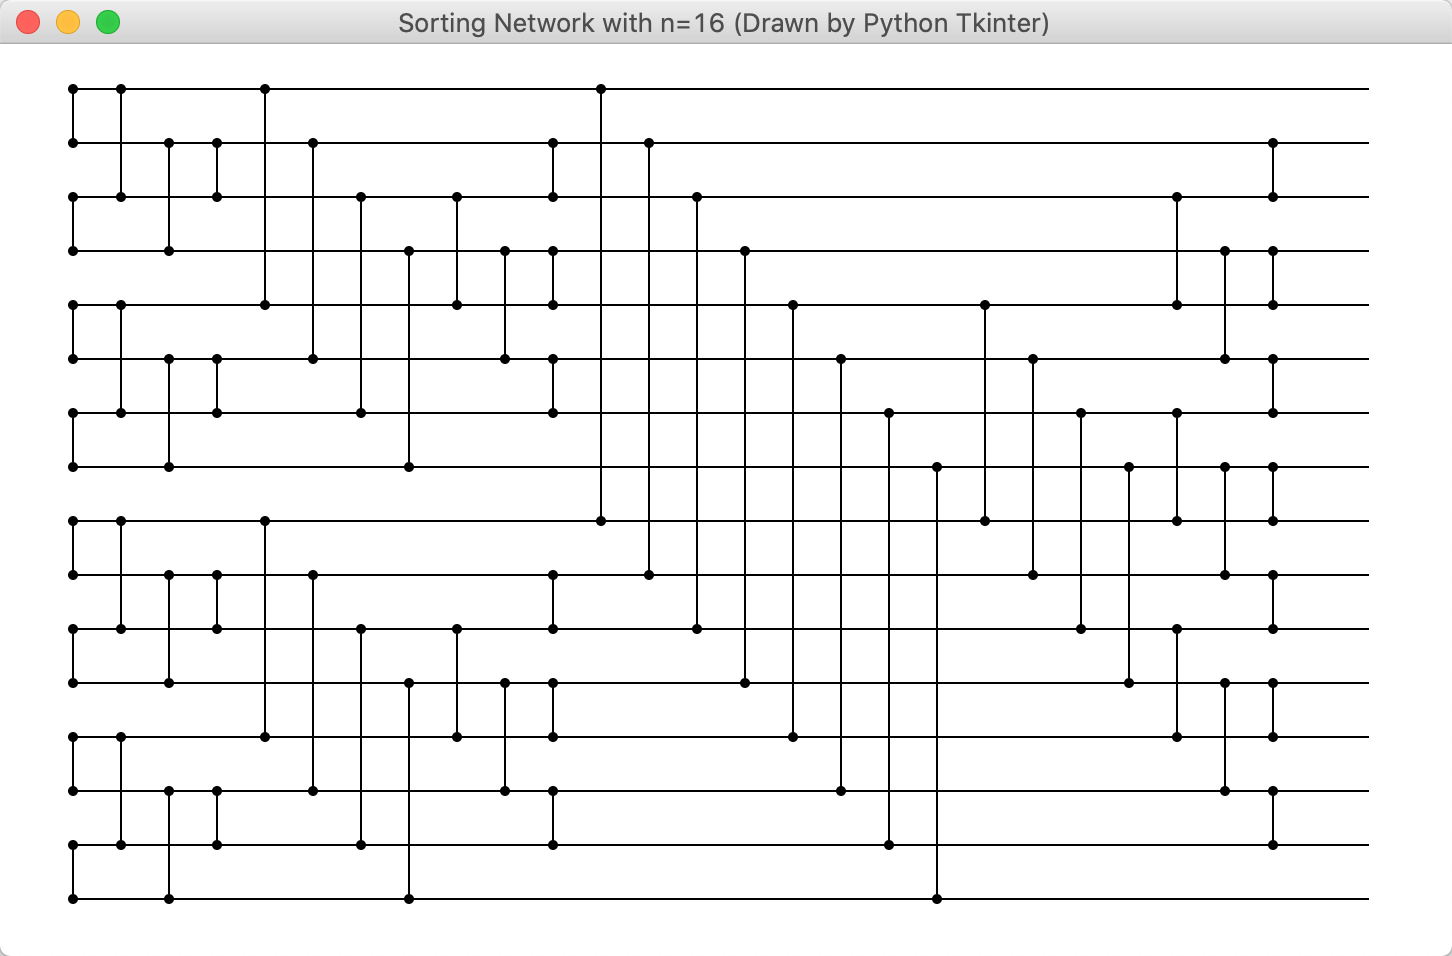
\includegraphics[scale=0.3]{2n=16} 
			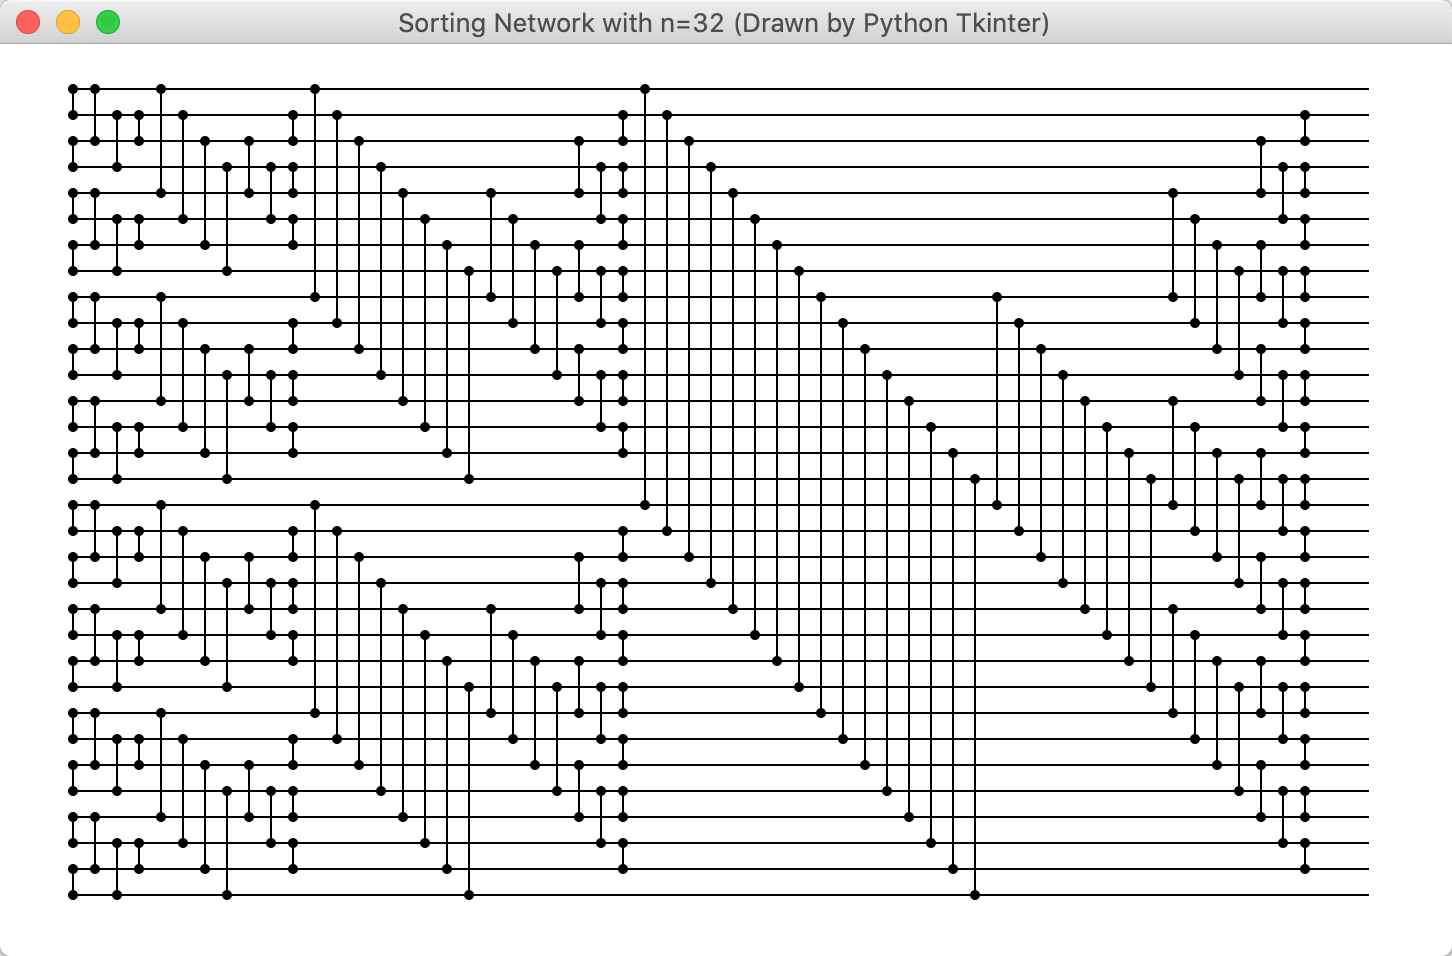
\includegraphics[scale=0.3]{2n=32} \\
			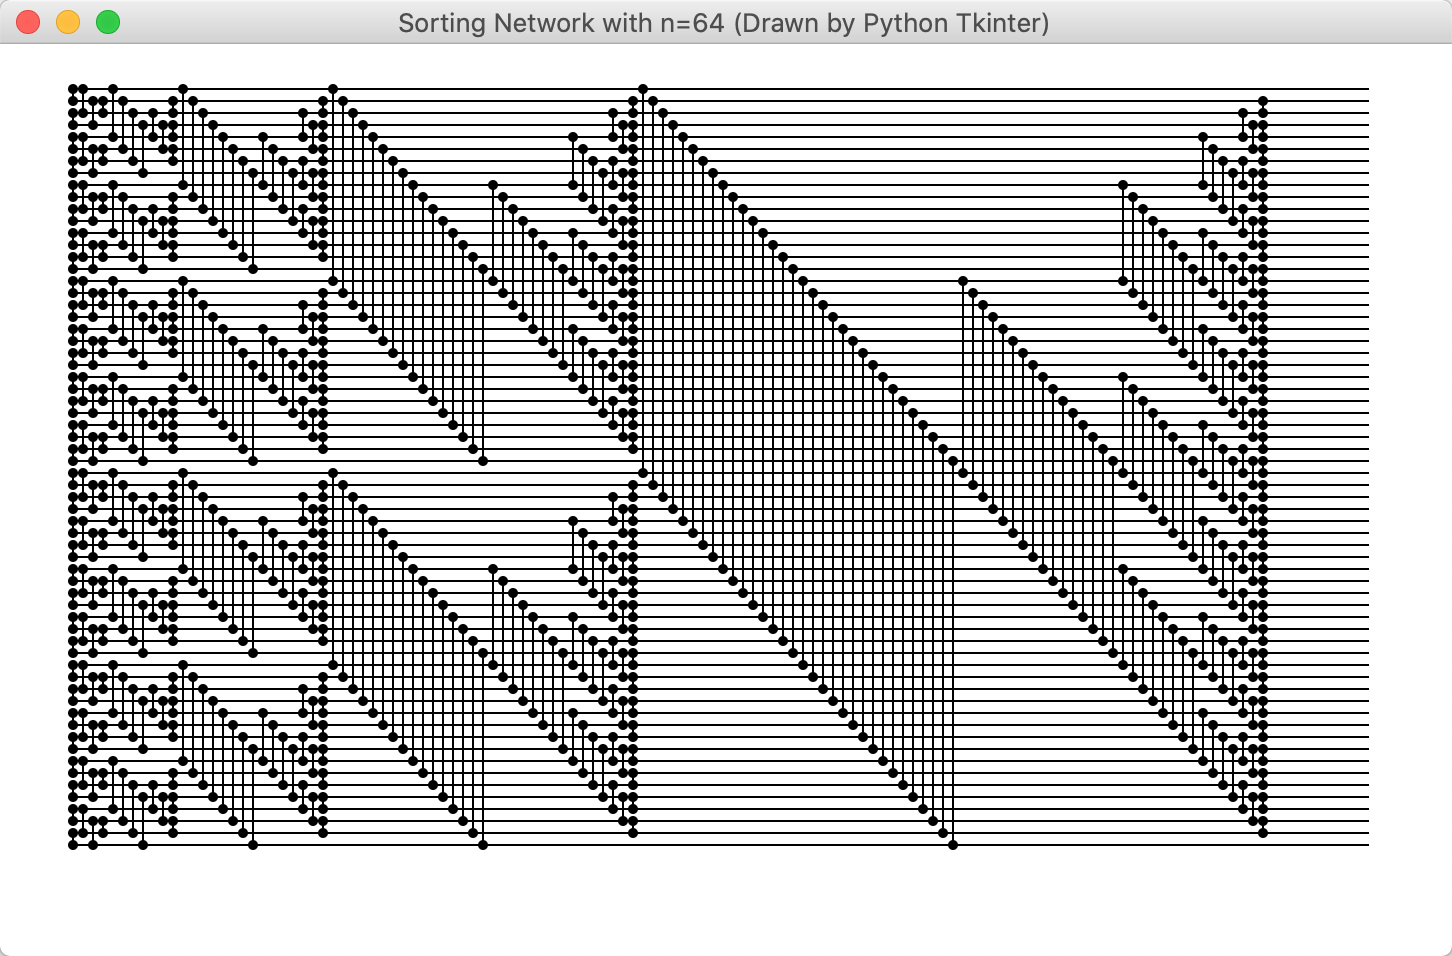
\includegraphics[scale=0.3]{2n=64} 
			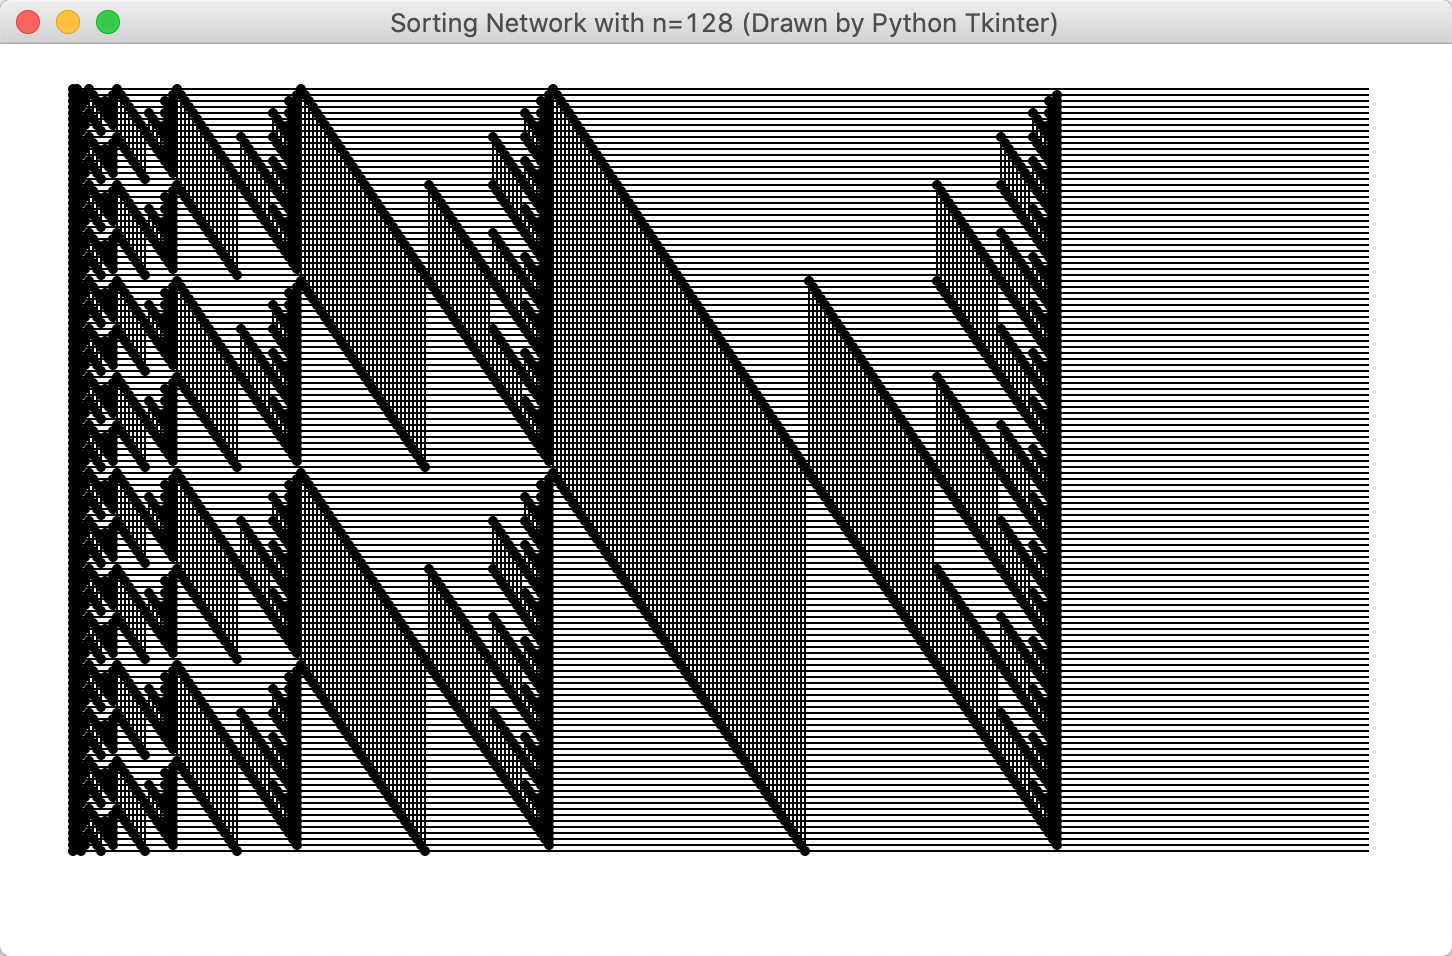
\includegraphics[scale=0.3]{2n=128}
			\item
			The depth of Sorter[$2n$] is given by the recurrence:
			\[
				D(2n) = 
				\begin{cases}
					1 \, & \text{for} \, n=1 \\
					D(n) + \log_{2} 2n \, & \text{for} \, n=2^k \, \text{and} \, k \geq 1
				\end{cases}
			\]
			whose solution is $D(2n) = \Theta (\log ^2 n)$.
			\item
			Firstly, we'll prove that the merging network works fine for $0$-$1$ sequences. \\
			Suppose that $\left\langle a_{1}, a_{2}, \ldots, a_{n}\right\rangle$ starts with $m_1$ $0$'s, $\left\langle a_{n+1}, a_{n+2}, \ldots, a_{2n}\right\rangle$ starts with $m_2$ $0$'s. Then $\left\langle a_{1}, a_{3}, \ldots, a_{2n-1}\right\rangle$ has $\lceil \frac{m_1}{2} \rceil + \lceil \frac{m_2}{2} \rceil$ $0$'s, while $\left\langle a_{2}, a_{4}, \ldots, a_{2n}\right\rangle$ has $\lfloor \frac{m_1}{2} \rfloor + \lfloor \frac{m_2}{2} \rfloor$ $0$'s. Hence the odd sequence has $0,1,\text{or } 2$ more $0$'s than the even one. \\
			After merging on both the odd and even sequences, $0$'s go up while $1$'s go down. If the odd sequence has $0$ or $1$ more $0$'s than the even one, the whole sequence is already merged. If the odd sequence had $2$ more $0$'s than the even one, the comparators between $a_{2i}$ and $a_{2i+1}$ ($i=1,2, \ldots, n-1$) will fix the problem, i.e., exchanging the $1$ of the even sequence and the $0$ of the odd sequence right below it. \\
			In conclusion, the merging network is correct for $0$-$1$ sequences. As \textit{\textbf{Zero-one principle}} indicates, the network sorts all sequences of arbitrary numbers correctly. 
		\end{enumerate}
	\end{solution}

\end{enumerate}

\vspace{20pt}

\textbf{Remark:} You need to include your .pdf, .tex and .py files (or other possible sources) in your uploaded .rar or .zip file.

%========================================================================
\end{document}
